\documentclass[tikz]{standalone}
\input{../tikz/plots_config.pgs}

\begin{document}

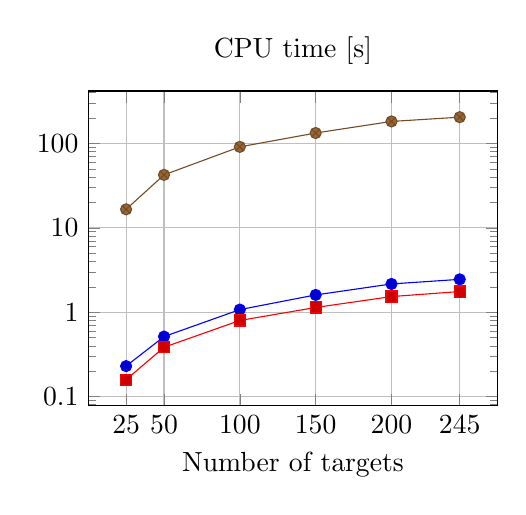
\begin{tikzpicture}
\begin{semilogyaxis}[%
log ticks with fixed point,
max space between ticks=20,
width=52mm,
height=40mm,
scale only axis,
xmin=0,
xmax=270,
xtick={25, 50, 100, 150, 200, 245},
xmajorgrids,
ymajorgrids,
title={CPU time [s]},
xlabel={Number of targets},
]
% Euclidean
\addplot coordinates{
	(25, 0.229706048965)
	(50, 0.51425909996)
	(100, 1.07467389107)
	(150, 1.60365986824)
	(200, 2.16413116455)
	(245, 2.45354890823)
};

% Max Joint Distance
\addplot coordinates{
	(25, 0.158663034439)
	(50, 0.384294986725)
	(100, 0.798450946808)
	(150, 1.13834905624)
	(200, 1.53367209435)
	(245, 1.7586209774)
};

% Linear Interpolation
\addplot coordinates{
	(25, 16.59339118)
	(50, 42.4946699142)
	(100, 91.2947571278)
	(150, 133.232317924)
	(200, 182.842684031)
	(245, 205.183601141)
};
\end{semilogyaxis}
\end{tikzpicture}

\end{document}
